%%%%%%%%%%%%%%%%%%%%%%%%%%%%%%%%%%%%%%%%%
% Short Sectioned Assignment
% LaTeX Template
% Version 1.0 (5/5/12)
%
% This template has been downloaded from:
% http://www.LaTeXTemplates.com
%
% Original author:
% Frits Wenneker (http://www.howtotex.com)
%
% License:
% CC BY-NC-SA 3.0 (http://creativecommons.org/licenses/by-nc-sa/3.0/)
%
%%%%%%%%%%%%%%%%%%%%%%%%%%%%%%%%%%%%%%%%%

%----------------------------------------------------------------------------------------
%	PACKAGES AND OTHER DOCUMENT CONFIGURATIONS
%----------------------------------------------------------------------------------------

\documentclass[paper=a4, fontsize=11pt]{scrartcl} % A4 paper and 11pt font size

\usepackage[T1]{fontenc} % Use 8-bit encoding that has 256 glyphs
\usepackage{fourier} % Use the Adobe Utopia font for the document - comment this line to return to the LaTeX default
\usepackage[english]{babel} % English language/hyphenation
\usepackage{amsmath,amsfonts,amsthm} % Math packages

\usepackage[colorinlistoftodos]{todonotes}
\usepackage{pifont}
\usepackage{mdframed,color}

\usepackage{graphicx}

\usepackage{lipsum} % Used for inserting dummy 'Lorem ipsum' text into the template

\usepackage{sectsty} % Allows customizing section commands
\allsectionsfont{\normalfont\scshape} % Make all sections left, the default font and small caps

\usepackage{fancyhdr} % Custom headers and footers
\pagestyle{fancyplain} % Makes all pages in the document conform to the custom headers and footers
\fancyhead[R]{A. Olson - H. Stanton} % No page header - if you want one, create it in the same way as the footers below
\fancyhead[L]{Stat775-HW3}
\fancyfoot[L]{} % Empty left footer
\fancyfoot[C]{} % Empty center footer
\fancyfoot[R]{\thepage} % Page numbering for right footer
\renewcommand{\headrulewidth}{0pt} % Remove header underlines
\renewcommand{\footrulewidth}{0pt} % Remove footer underlines
\setlength{\headheight}{13.6pt} % Customize the height of the header

\numberwithin{equation}{section} % Number equations within sections (i.e. 1.1, 1.2, 2.1, 2.2 instead of 1, 2, 3, 4)
\numberwithin{figure}{section} % Number figures within sections (i.e. 1.1, 1.2, 2.1, 2.2 instead of 1, 2, 3, 4)
\numberwithin{table}{section} % Number tables within sections (i.e. 1.1, 1.2, 2.1, 2.2 instead of 1, 2, 3, 4)

\setlength\parindent{0pt} % Removes all indentation from paragraphs - comment this line for an assignment with lots of text

\newtheoremstyle{statement}{3pt}{3pt}{}{}{\bfseries}{:}{.5em}{}

\theoremstyle{statement}
\newtheorem*{atmProp}{Proposition}

\newenvironment{atmProof}{\noindent\ignorespaces\paragraph{Proof:}}{\hfill \ding{122}\par\noindent}

%----------------------------------------------------------------------------------------
%	TITLE SECTION
%----------------------------------------------------------------------------------------

\newcommand{\horrule}[1]{\rule{\linewidth}{#1}} % Create horizontal rule command with 1 argument of height

\newcommand{\N}{\mathbb{N}}
\newcommand{\Z}{\mathbb{Z}}
\newcommand{\R}{\mathbb{R}}
\newcommand{\Q}{\mathbb{Q}}
\newcommand{\Pow}{\mathcal{P}}
\newcommand{\Prime}{\mathbb{P}}
\newcommand{\C}{\mathbb{C}}

\newcommand{\sand}{\wedge}
\newcommand{\sor}{\vee}

\newcommand{\lb}{\lbrace}
\newcommand{\rb}{\rbrace}

\title{	
\normalfont \normalsize 
\textsc{Statistical Machine Learning} \\ [25pt] % Your university, school and/or department name(s)
\horrule{0.5pt} \\[0.4cm] % Thin top horizontal rule
\huge Stat 775 HW 4 \\ % The assignment title
\horrule{2pt} \\[0.5cm] % Thick bottom horizontal rule
}

\author{Andrew Olson - Harrison Stanton} % Your name

\date{\normalsize\today} % Today's date or a custom date

\begin{document}

\maketitle % Print the title

%----------------------------------------------------------------------------------------
%	PROBLEM 1
%----------------------------------------------------------------------------------------

\section{Problem Set}
\subsection{Exercise 3.12}
Show that the ridge regression estimates can be obtained by ordinary least squares regression on an augmented data set. We augment the centered matrix \textbf{X} with \textit{p} additional rows $\sqrt{\lambda}$\textbf{I}, and augment \textbf{y} with \textit{p} zeros.\\
\[
    \hat{X} = 
    \begin{bmatrix}
        X\\
        \sqrt{\lambda} I_{pxp}        
    \end{bmatrix}    
    \hat{Y} = 
    \begin{bmatrix}
        Y\\
        \mathcal O_{px1}       
    \end{bmatrix}
\]

By introducing artificial data having response value zero, the fitting procedure is forced to shrink the coefficients toward zero. This is ...  that satisfy them.\\

\[
    \hat{\beta}_{LS} = (\hat{X}^T\hat{X} + \lambda I_{pxp})^{-1}\hat{X}^T\hat{Y}
\]
\[
    \hat{X}^T\hat{X} = 
    \begin{bmatrix}
        X^T & \sqrt{\lambda}I_{pxp}
    \end{bmatrix}
    \begin{bmatrix}
        X\\
        \sqrt{\lambda}I_{pxp}
    \end{bmatrix}
    = X^X + \lambda I_{pxp}
\]
\[
    \hat{X}^T\hat{Y} = 
    \begin{bmatrix}
        X^T & \sqrt{\lambda}
    \end{bmatrix}
    \begin{bmatrix}
        Y\\
        \mathcal{O}_{px1}    
    \end{bmatrix}
    = X^TY
\]
\[
    \hat{\beta}_{LS} = (X^TX + \lambda_{pxp})^{-1}X^TY
\]
\subsection{Code}

The assignment was to use Fisher Discriminators to distinguish between 2 and 3, 4 and 5, and 7 and 9 from the Zip code digit data given by the book. \\

The only real issues were related to trying to get Python and Numpy to get the dimensionality of arrays and matrices correct. Beyond that, dealing with the occasional singular matrix was the only other excitement. The following give the output for both the training and the test data.\\

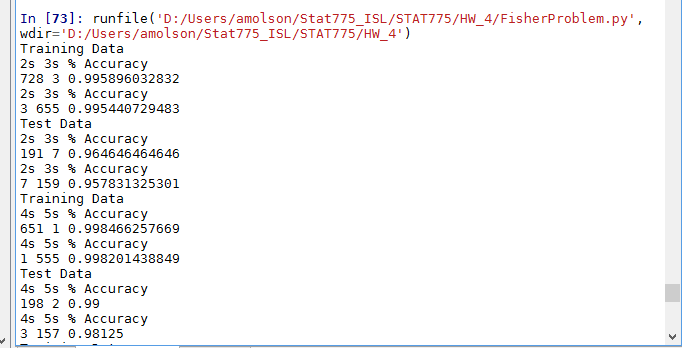
\includegraphics[scale=0.6]{Fisher1.png}

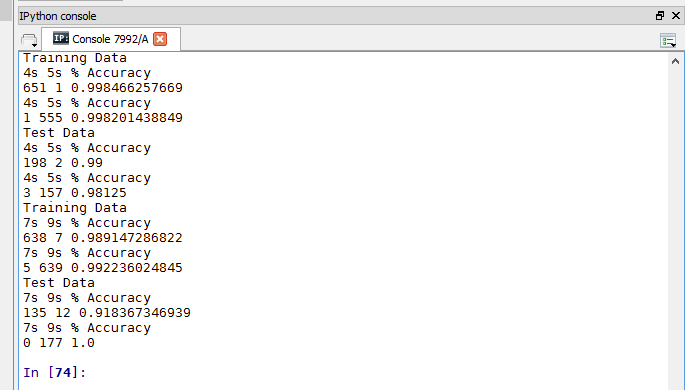
\includegraphics[scale=0.6]{Fisher2.png}  

\pagebreak
Here is the actual code. \\

\begin{verbatim}
#23, 45, 79

import numpy as np

import matplotlib.pyplot as plt
import numpy.linalg as la

import math

sigma = np.load("sigmazip.npy")
mu = np.load("muzip.npy")

training = np.load("trainingzip.npy")
testing = np.load("testingzip.npy")

#Check any pairs you like.
Numbers = [(2, 3), (4, 5), (7, 9)]

in_array = testing

distancearray = []

tracking = []

def probofx(x, mu, sigma):
    inter = 1.0/(math.sqrt(2 * math.pi * sigma))
    expon = (-0.5 * (x - mu) ** 2)/(sigma ** 2)
    return inter * math.exp(expon)

def buildu(sigma, mu, first, second):
    """Builds a based on sigma, mu, first and second values under 
    investigation"""
    #Prebuild arrays and catch singular matrix and try epsilon I matrix
    try:
        sigmasub = np.matrix(la.inv(sigma[second] + sigma[first]))
    except np.linalg.LinAlgError:
        sigmasub = np.matrix(la.inv(sigma[second] + sigma[first] + 
            np.identity(len(sigma[second]))*np.finfo(float).eps))
    
    musub = np.matrix(mu[second] - mu[first])
    
    #Put them together and then normalize to unit vector. a \equiv u
    a = sigmasub * np.transpose(musub)    
    a = np.divide(a, la.norm(a))
    
    return a

#Change this value to test the pairs in Numbers. 0 index
for problem in range(3):

    first = Numbers[problem][0]
    second = Numbers[problem][1]
    
    points = [first, second]
            
    a = buildu(sigma, mu, first, second)
    
    #Python was being a butt so I had to go through this little song and 
    #dance to get floats in the array, not an array of array points. Don't ask.
    aprime = []
    for i in a:
        aprime.append(float(i))
    
    train = []
    test = []
    
    mean = [[], []]
    sd = [[], []]
    count = [0, 0]
    
    #Build empty array
    for i in range(10):
        train.append([])    
    #Add training data to matrix it belongs in
    for i in training:
        train[i[1]].append(i[0])

    #Build empty array
    for i in range(10):
        test.append([])    
    #Add training data to matrix it belongs in
    for i in testing:
        test[i[1]].append(i[0])              
    
    #This was getting silly since note they use different mu.        
    mean[0] = np.dot(mu[first], aprime)
    sd[0] = math.sqrt(float(np.transpose(a) * sigma[first] * a))
    
    mean[1] = np.dot(mu[second], aprime)
    sd[1] = math.sqrt(float(np.transpose(a) * sigma[second] * a))
    
    print "Training Data"
    #And this is it
    for order in points:
        count = [0, 0]
        for i in range(len(train[order])):
            
            ifis = [0, 0]
            whichvalue = np.dot(train[order][i], aprime)
            ifis[0] = probofx(whichvalue, mean[0], sd[0])
            
            ifis[1] = probofx(whichvalue, mean[1], sd[1])
        
            if ifis[0] > ifis[1]:
                count[0] += 1
            else:
                count[1] += 1
                
        if order == first:
            print str(first) + 's', str(second) + 's', '% Accuracy'
            print count[0], count[1], float(count[0])/float(count[0]+count[1])
        else:
            print str(first) + 's', str(second) + 's', '% Accuracy'
            print count[0], count[1], float(count[1])/float(count[0]+count[1])
            
    print "Test Data"
    #And this is it
    for order in points:
        count = [0, 0]
        for i in range(len(test[order])):
            
            ifis = [0, 0]
            whichvalue = np.dot(test[order][i], aprime)
            ifis[0] = probofx(whichvalue, mean[0], sd[0])
            
            ifis[1] = probofx(whichvalue, mean[1], sd[1])
        
            if ifis[0] > ifis[1]:
                count[0] += 1
            else:
                count[1] += 1
                
        if order == first:
            print str(first) + 's', str(second) + 's', '% Accuracy'
            print count[0], count[1], float(count[0])/float(count[0]+count[1])
        else:
            print str(first) + 's', str(second) + 's', '% Accuracy'
            print count[0], count[1], float(count[1])/float(count[0]+count[1])
\end{verbatim}
\end{document}